\documentclass{article}
\usepackage{amsmath}
\usepackage{tikz}
\usetikzlibrary{decorations.pathmorphing}

\begin{document}

\begin{center}
    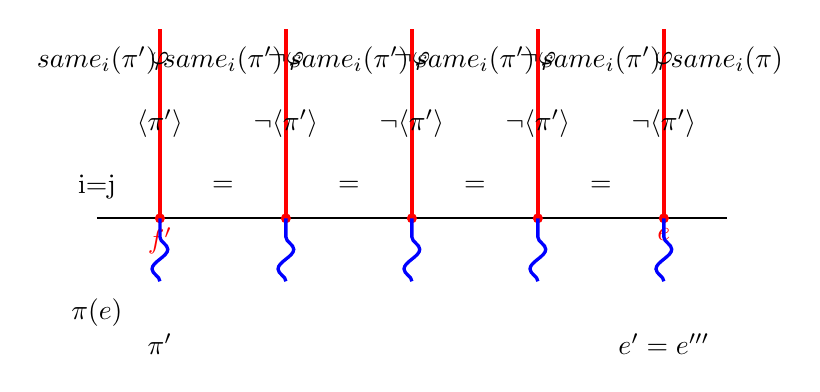
\begin{tikzpicture}[scale=0.8]
        % Draw the horizontal line
        \draw[thick] (-5,0) -- (5,0);
        
        % Mark the points with red circles
        \filldraw[red] (-4,0) circle (2pt) node[below] {$f'$};
        \filldraw[red] (-2,0) circle (2pt) node[below] {};
        \filldraw[red] (0,0) circle (2pt) node[below] {};
        \filldraw[red] (2,0) circle (2pt) node[below] {};
        \filldraw[red] (4,0) circle (2pt) node[below] {$e$};
        
        % Draw the vertical lines
        \draw[very thick, red] (-4,0) -- (-4,3);
        \draw[very thick, red] (-2,0) -- (-2,3);
        \draw[very thick, red] (0,0) -- (0,3);
        \draw[very thick, red] (2,0) -- (2,3);
        \draw[very thick, red] (4,0) -- (4,3);
        
        % Add the labels for the vertical lines
        \node at (-4,1.5) {$\langle\pi'\rangle$};
        \node at (-2,1.5) {$\neg\langle\pi'\rangle$};
        \node at (0,1.5) {$\neg\langle\pi'\rangle$};
        \node at (2,1.5) {$\neg\langle\pi'\rangle$};
        \node at (4,1.5) {$\neg\langle\pi'\rangle$};
        
        % Add the labels for the red circles
        \node at (-4,2.5) {$\varphi$};
        \node at (-2,2.5) {$\neg\varphi$};
        \node at (0,2.5) {$\neg\varphi$};
        \node at (2,2.5) {$\neg\varphi$};
        \node at (4,2.5) {$\varphi$};
        
        % Draw the zigzag lines
        \draw[blue, very thick, decorate, decoration={snake, amplitude=1mm, segment length=5mm}] (-4,-1) -- (-4,0);
        \draw[blue, very thick, decorate, decoration={snake, amplitude=1mm, segment length=5mm}] (-2,-1) -- (-2,0);
        \draw[blue, very thick, decorate, decoration={snake, amplitude=1mm, segment length=5mm}] (0,-1) -- (0,0);
        \draw[blue, very thick, decorate, decoration={snake, amplitude=1mm, segment length=5mm}] (2,-1) -- (2,0);
        \draw[blue, very thick, decorate, decoration={snake, amplitude=1mm, segment length=5mm}] (4,-1) -- (4,0);
        
        % Add the labels for the zigzag lines
        \node at (-4,-2) {$\pi'$};
        \node at (4,-2) {$e'=e'''$};
        
        % Add the text above the horizontal line
        \node at (-5,0.5) {i=j};
        \node at (-3,0.5) {$=$};
        \node at (-1,0.5) {$=$};
        \node at (1,0.5) {$=$};
        \node at (3,0.5) {$=$};
        
        % Add the labels for the "same" conditions
        \node at (5,2.5) {$same_i(\pi)$};
        \node at (-5,2.5) {$same_i(\pi')$};
        \node at (-3,2.5) {$same_i(\pi')$};
        \node at (-1,2.5) {$same_i(\pi')$};
        \node at (1,2.5) {$same_i(\pi')$};
        \node at (3,2.5) {$same_i(\pi')$};
        
        % Add the label for the bottom left corner
        \node at (-5,-1.5) {$\pi(e)$};
    \end{tikzpicture}
\end{center}

\textbf{Case $\pi=\prevon{i}{\varphi}\cdot\pi'$ and $t,e'' \models \phi$}

\end{document}